\section{Skeleton}

\textit{Can a neural network learn to scan Hexameters?}\\

1. Approach using HMM
2. Approach using CRF
3. Approach using LSTM
4. Approach using ELECTRA

\textbf{What is the effect of different genres}
For Hexameter, two different genres: saturae and epic. No noticeable difference detected.

Clustering texts: agglomerative clustering: create tree from Kestemont


\textbf{What is the effect of different time periods}
No difference detected. Virgil works fine on Iuvenal.


Notes:
normalise results. same corpus size ovid compared to same size virgil

\textbf{Flair}
What is the effect of different word representations?
  Strings, hashes, syllable embeddings, char/syll/word embeddings
  Different context windows (5), dimensions (100-300), no mincount 
  fasttext (autovocab), glove, word2vec
    cluster these vectors using PCA: are clusters logial and relevant to our task? syntactical and semantical?

\textit{How well do these networks generalise to other meters?}
Elegiac, Iambic trimeter, anapest, trochaic tetrameter, polymetrum, hendycasyllabi

\newpage

\subsection{Conditional Random Fields}

Notes:
\begin{enumerate}
  \item Passing only syllables gave lower accuracy (between 1 and 5\%)
  \item More features like diphthongs or consonants did not improve accuracy
  \item No time era difference detected. Virgil works fine on Iuvenal.
  \item For Hexameter, two different genres: saturae and epic. No noticeable difference detected.
  \item Kestemont did detect genres
\end{enumerate}

\begin{lstlisting}[language=Python, caption=Python example]
    features = {
        'bias': 1.0,
        '0:syllable' : word, # just take the entire syllable
        '0:last_3_char': word[-2:], # Take last 2 characters
        '0:last_2_char': word[-1:], # Take last 1 characters
    }
    # Check if we are at the beginning of the sentence
    if i == 0:
        features['BOS'] = True # This should always be long
    # Gather features from the previous word
    if i > 0:
        previous_word = sent[i-1][0]
        features.update({
            '-1:word': previous_word,
            '-1:last_1_char': previous_word[-1:],
            '-1:last_2_char': previous_word[-2:],
        })
    # Gather features from the next word
    if i < len(sent)-1:
        next_word = sent[i+1][0]
        features.update({
            '+1:word': next_word,
            '+1:first_1_char': next_word[:1],
            '+1:first_2_char': next_word[:2],
        })
    else:
        features['EOS'] = True # This will be an anceps
\end{lstlisting}


\begin{figure}[H]
    \centering
    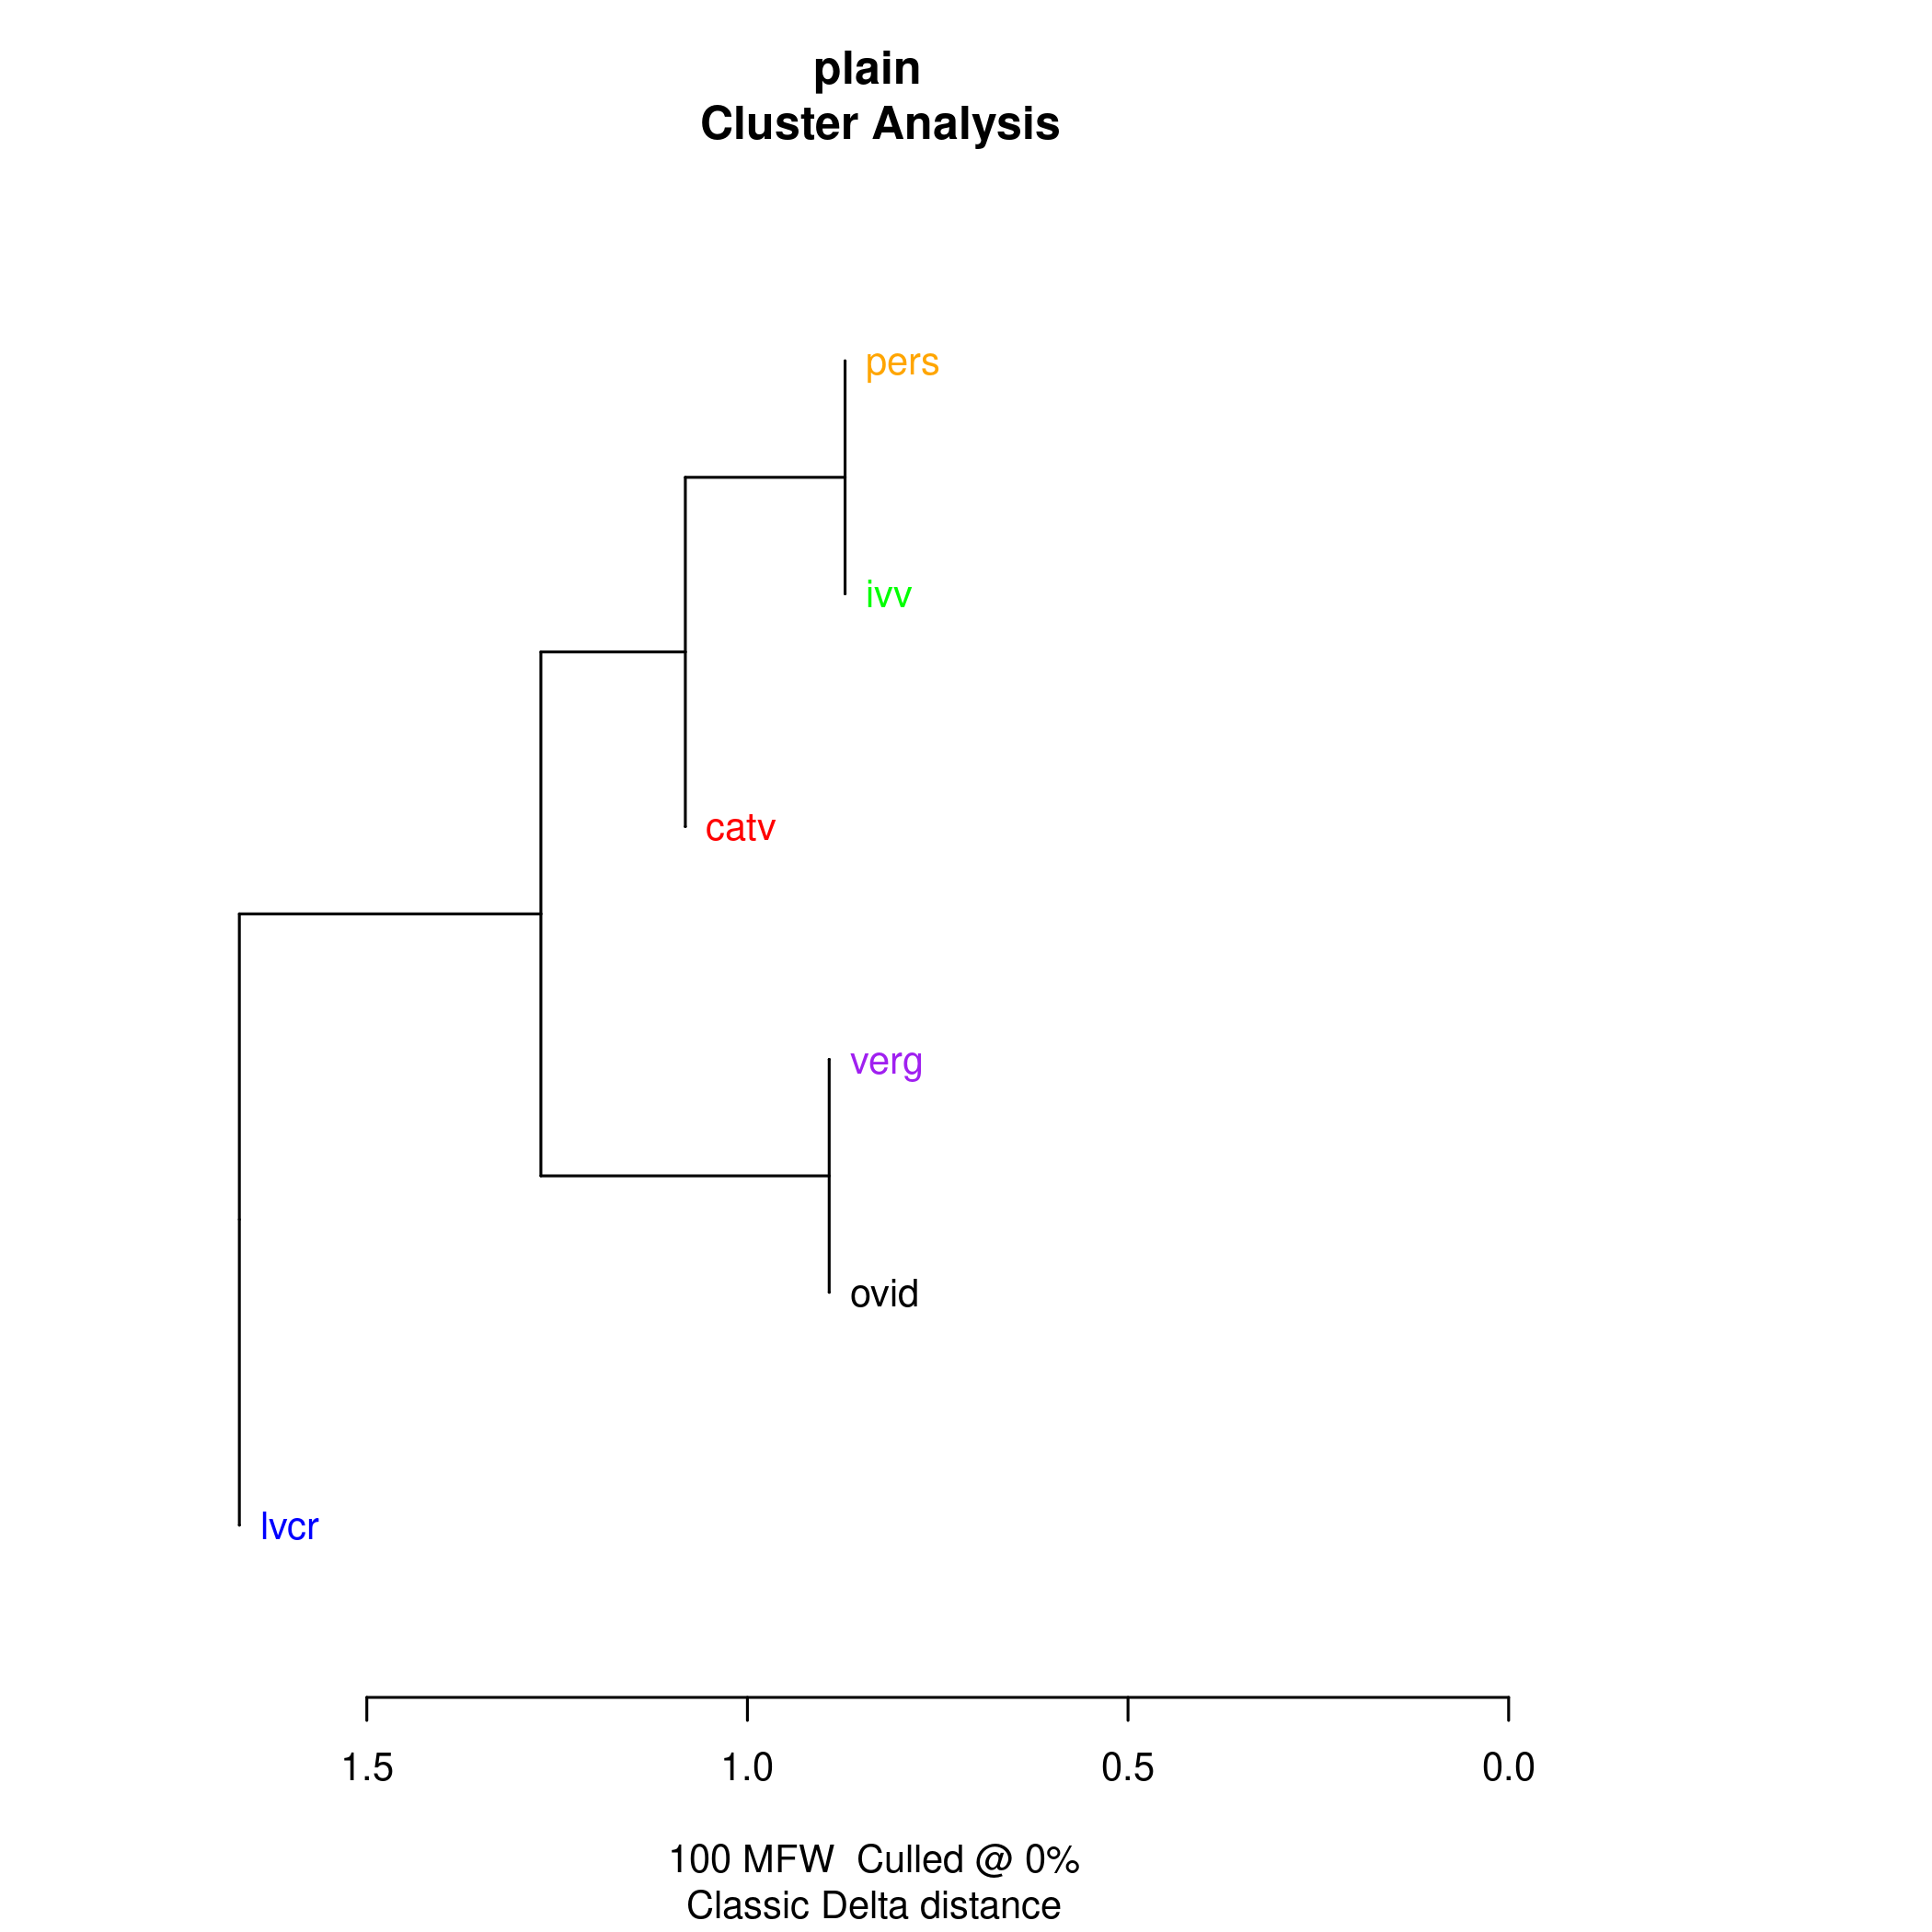
\includegraphics[width=0.95\textwidth]{img/hexameter_kestemont_tree.png}

    \caption{Hexameter texts clustering.}
    \label{fig:exp_architecture}
\end{figure}

\begin{figure}[H]
    \centering
    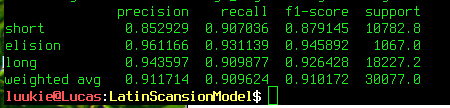
\includegraphics[width=0.95\textwidth]{img/crf/crf_confusion_matrix.png}

    \caption{CRF confusion matrix for Virgil's Aeneid.}
    \label{fig:exp_architecture}
\end{figure}

\newpage

\begin{figure}[H]
    \centering
    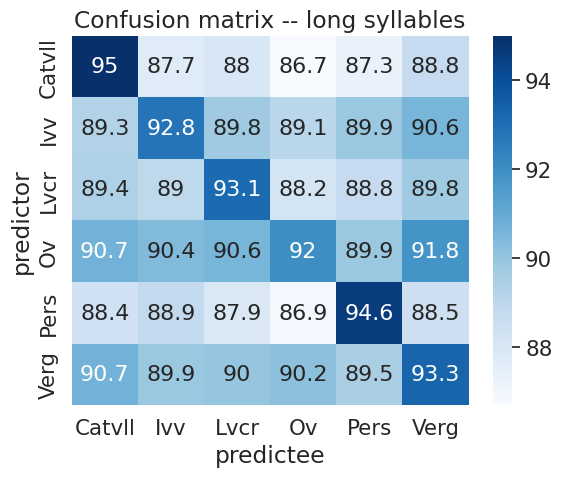
\includegraphics[width=0.48\textwidth]{img/crf/crf_label_accuracy_long.png}
    \quad
    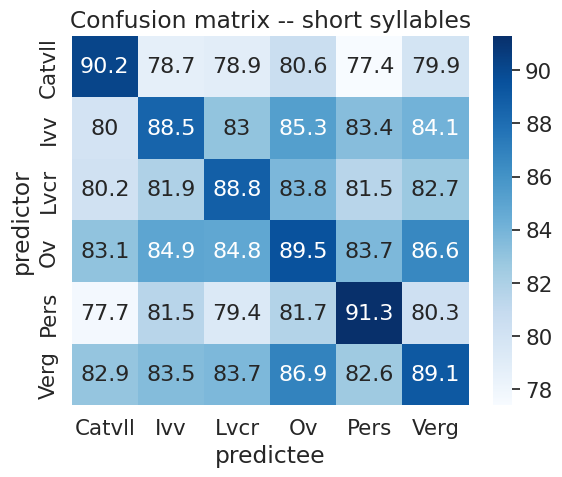
\includegraphics[width=0.48\textwidth]{img/crf/crf_label_accuracy_short.png}

    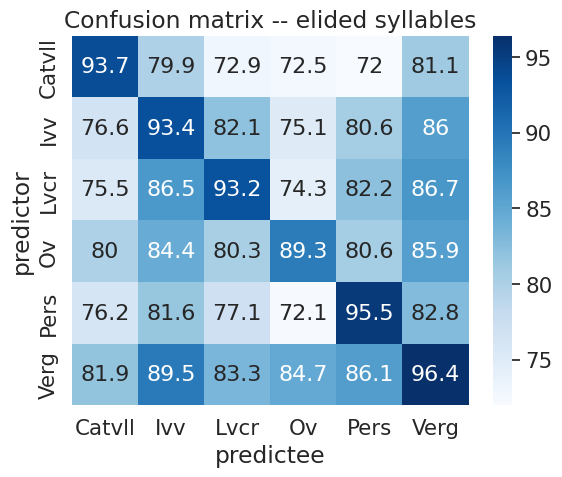
\includegraphics[width=0.48\textwidth]{img/crf/crf_label_accuracy_elision.png}
        % \quad
        % \includegraphics[width=0.48\textwidth]{img/task1_loss.png}

    % \captionsetup{justification=centering}
    \caption{CRF label accuracy for hexameter texts.}
    \label{fig:exp_architecture}
\end{figure}

\newpage
\subsection{LSTM}
\begin{enumerate}
  \item Syllables encoded with integers. Five labels: long, short, elision, space and padding.
	\item 25 epochs used, bi-directional LSTM, very simple.
	\item LSTM has extremely high accuracy within author if text is larger than 1000 lines.
	\item Transferability between authors is better than CRF.
	\item As with CRF, texts have to be larger than 1000 lines to achieve a nice accuracy.
    \item 25 epochs does seem to overfit slightly. Researching 10 epochs now.
    \item LSTM does also work on Pentameters, as seen by graph \ref{fig:exp_elegiac}.
    \item More lines is beneficial. Highest average accuracy with Hex + Ele model.
    \item LSTM trained on Hexameter and Pentameter can scan both. Also, a model trained on Hexameter + Pentameter can scan Hexameter texts better than a model purely trained on Hexameter. Same holds for Elegiac.
\end{enumerate}

\begin{figure}[H]
    \centering
    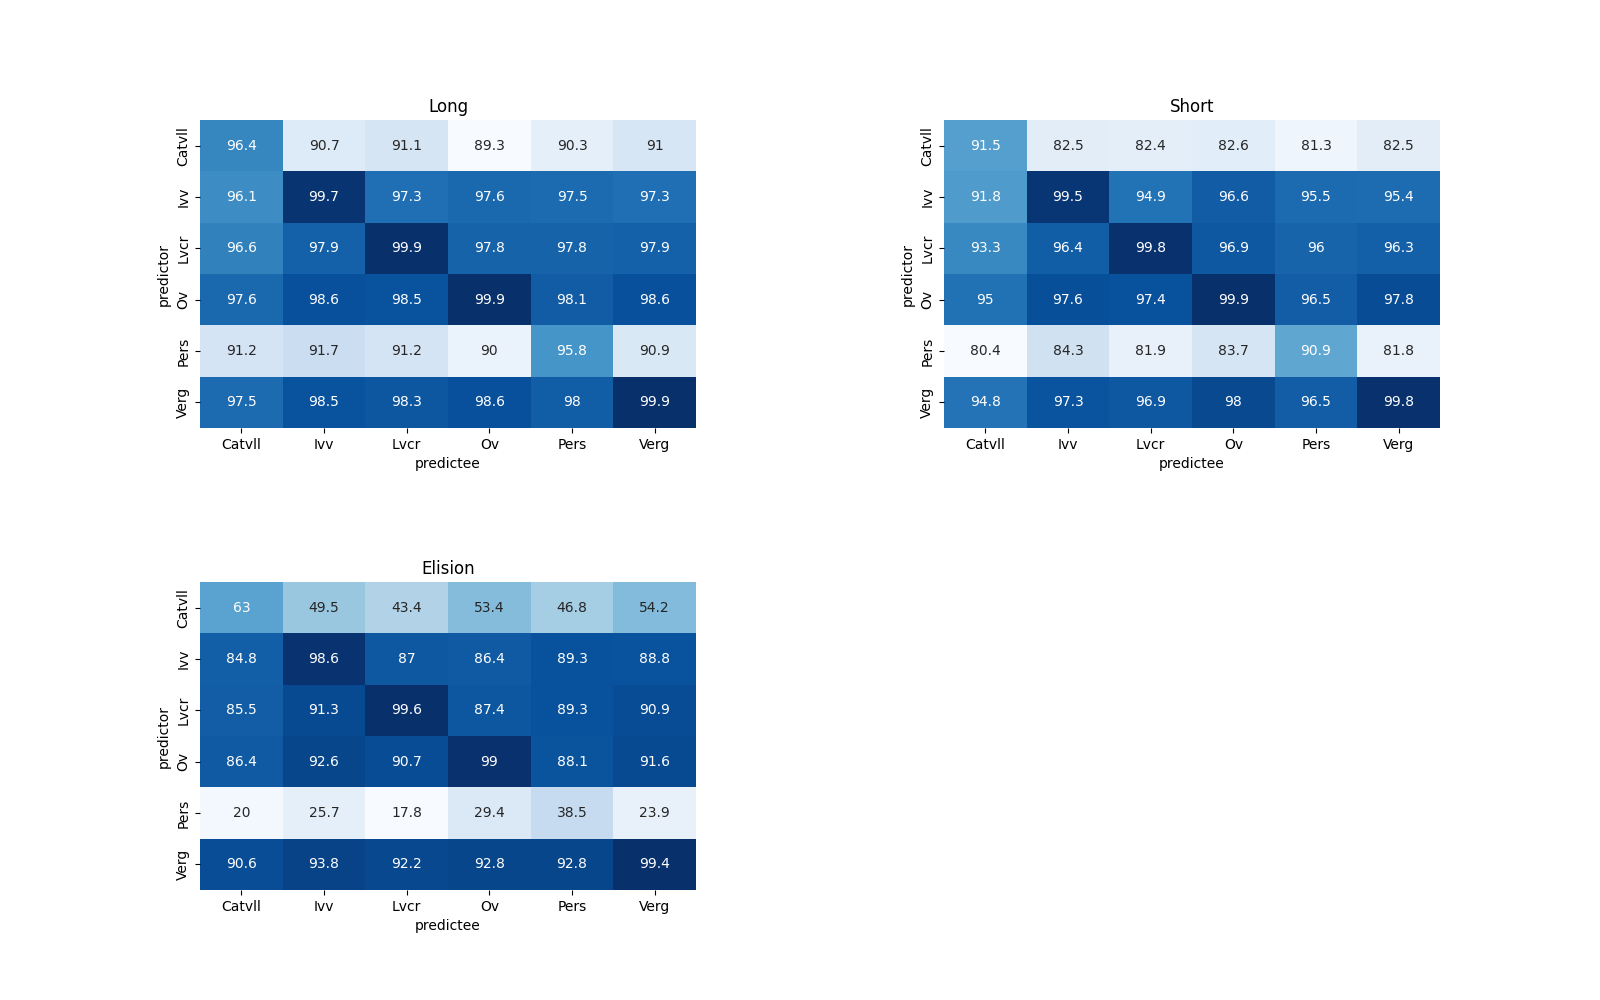
\includegraphics[width=1\textwidth]{img/lstm/lstm_hexameter_experiment.png}
    % \captionsetup{justification=centering}
    \caption{LSTM label accuracy for hexameter texts.}
    \label{fig:exp_architecture}
\end{figure}

\begin{figure}[H]
    \centering
    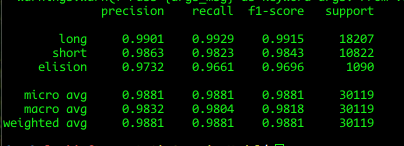
\includegraphics[width=0.95\textwidth]{img/lstm/lstm_confusion_matrix.png}

    \caption{LSTM confusion matrix for Virgil's Aeneid (10 epochs).}
    \label{fig:exp_architecture}
\end{figure}

\begin{figure}[H]
    \centering
    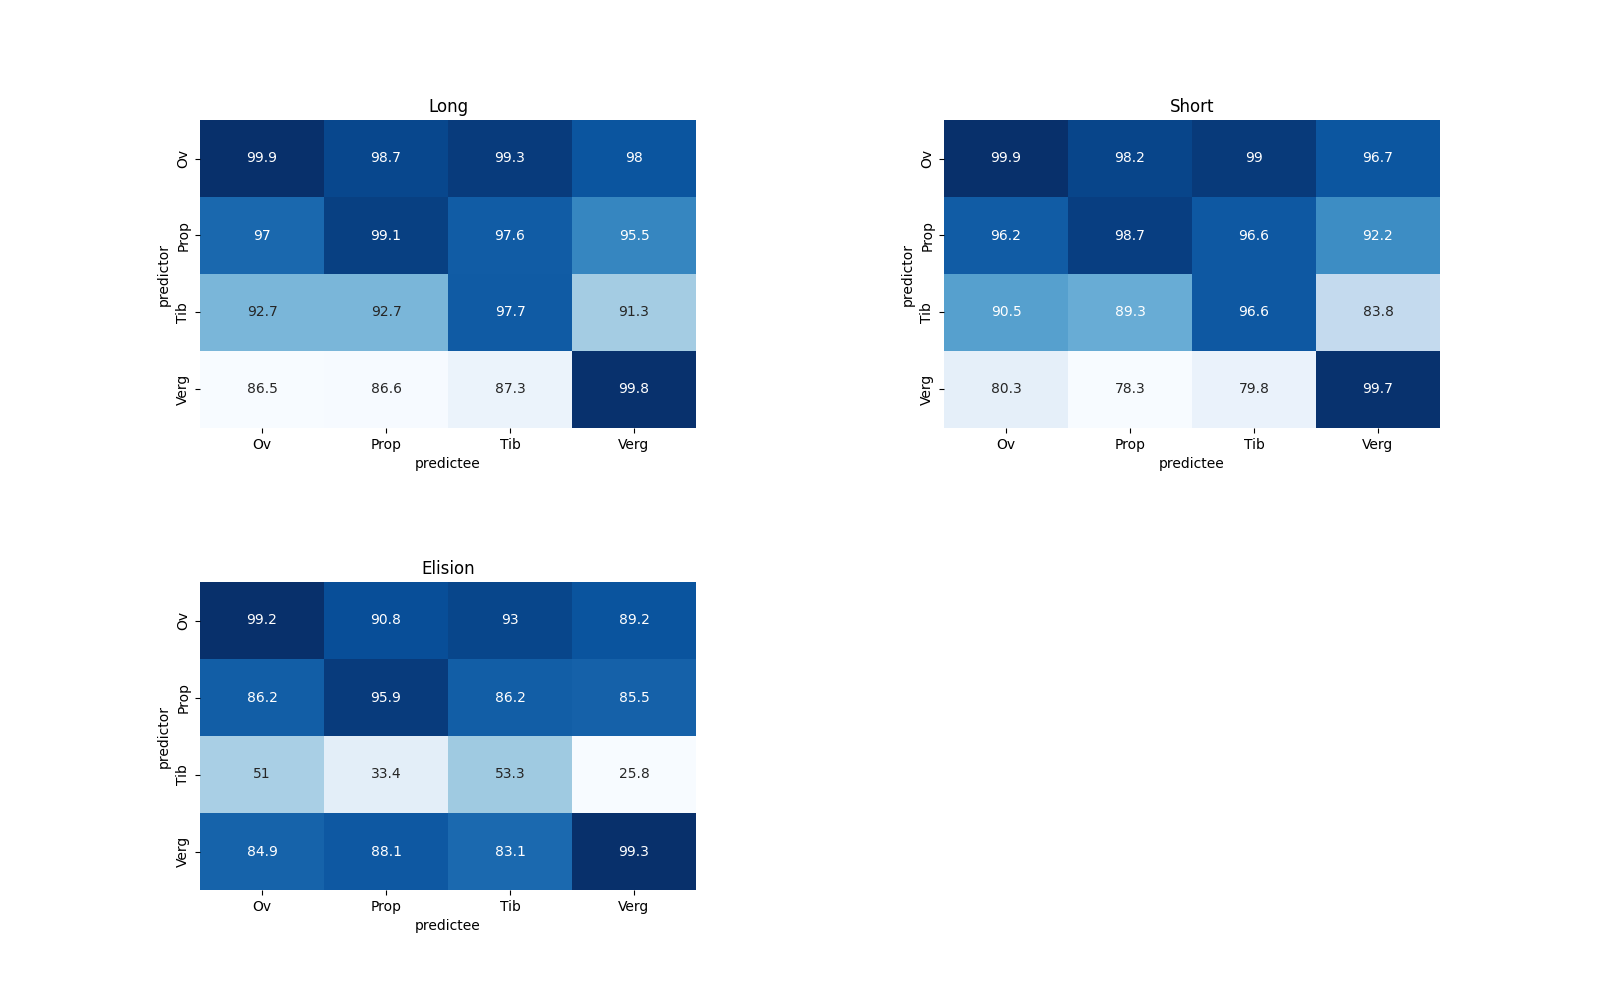
\includegraphics[width=0.95\textwidth]{img/lstm/lstm_label_accuracy_elegiac.png}

    \caption{LSTM label accuracy for elegiac texts.}
    \label{fig:exp_elegiac}
\end{figure}

% \begin{figure}[H]
%     \centering
%     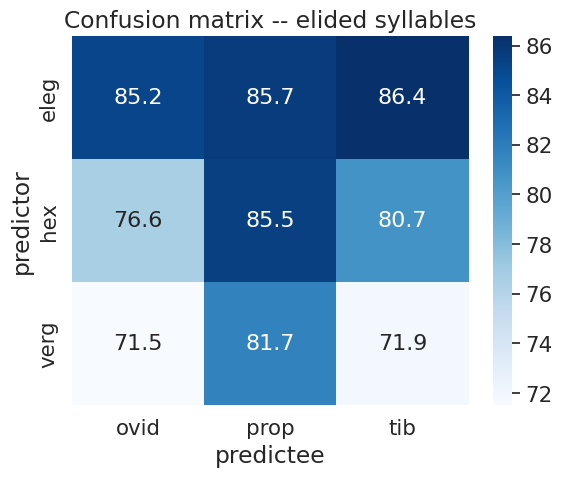
\includegraphics[width=0.48\textwidth]{img/lstm/lstm_label_accuracy_transfer_elision.png}
%     \quad
%     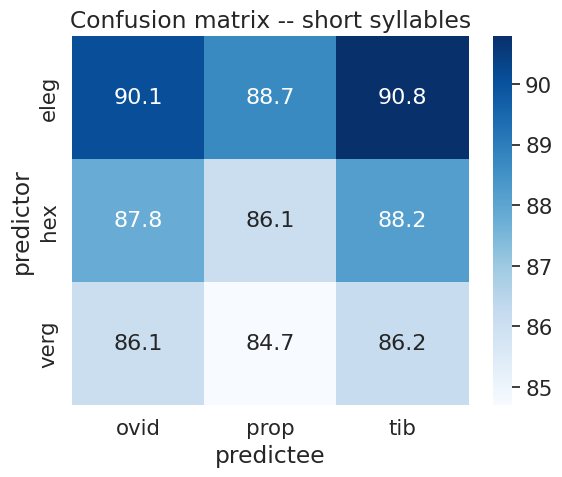
\includegraphics[width=0.48\textwidth]{img/lstm/lstm_label_accuracy_transfer_short.png}

%     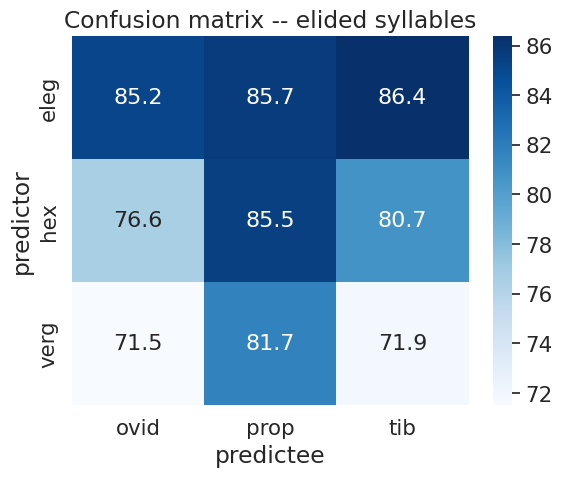
\includegraphics[width=0.48\textwidth]{img/lstm/lstm_label_accuracy_transfer_elision.png}
%         % \quad
%         % \includegraphics[width=0.48\textwidth]{img/task1_loss.png}

%     % \captionsetup{justification=centering}
%     \caption{LSTM label accuracy when combining hexameter and elegiac texts.}
%     \label{fig:exp_architecture}
% \end{figure}

\begin{figure}[H]
    \centering
    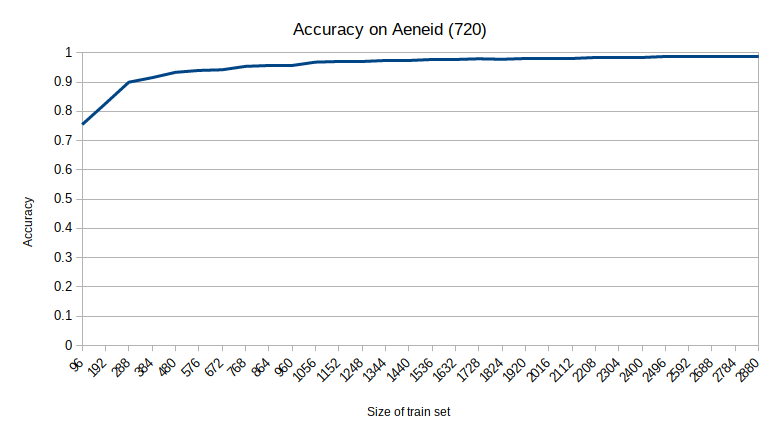
\includegraphics[width=0.95\textwidth]{img/lstm/lstm_minimum_train_set.png}

    \caption{LSTM minimum train size for acceptable accuracy.}
    \label{fig:exp_architecture}
\end{figure}

\begin{figure}[H]
    \centering
    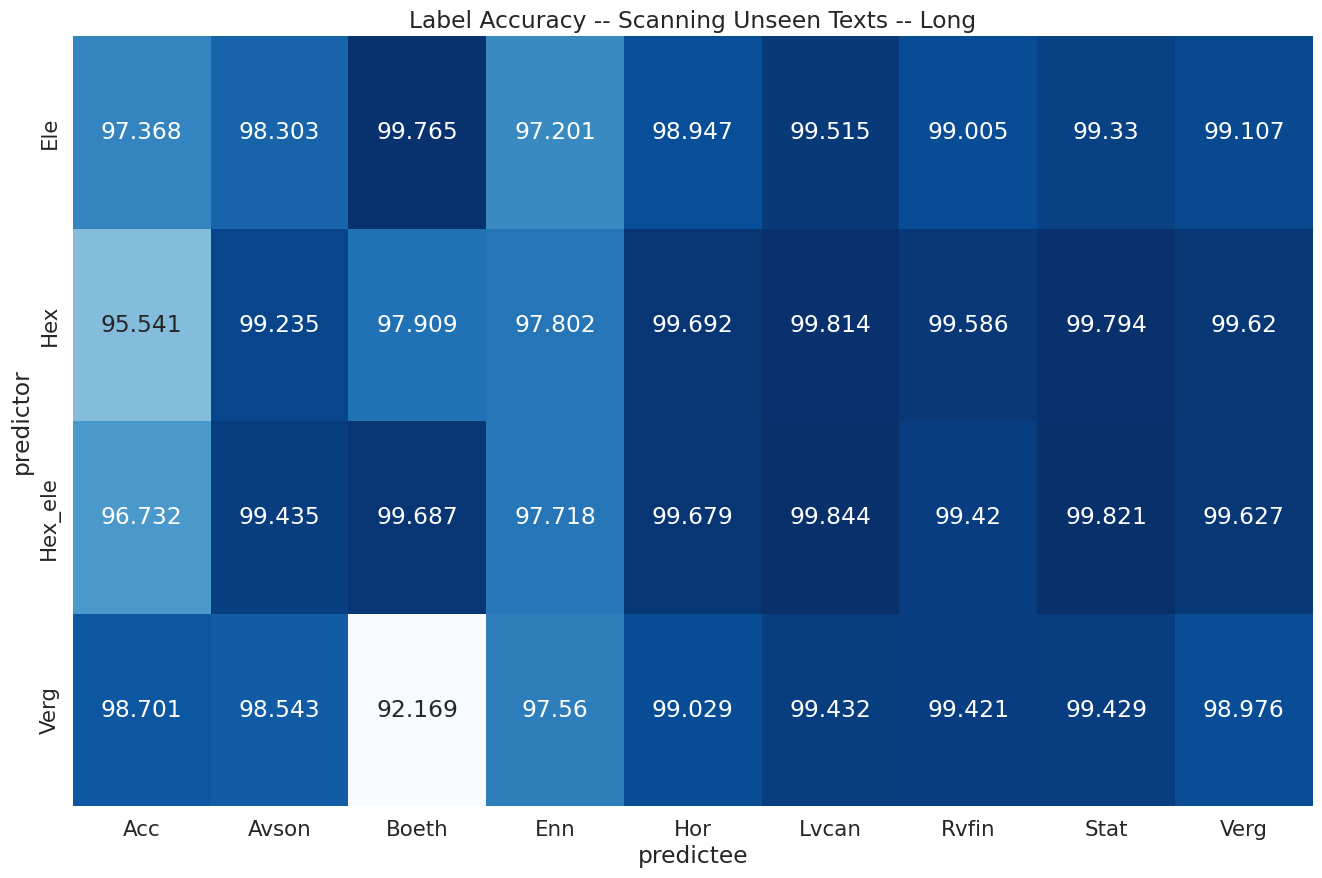
\includegraphics[width=0.48\textwidth]{img/lstm/lstm_unseen_texts-long.png}
    \quad
    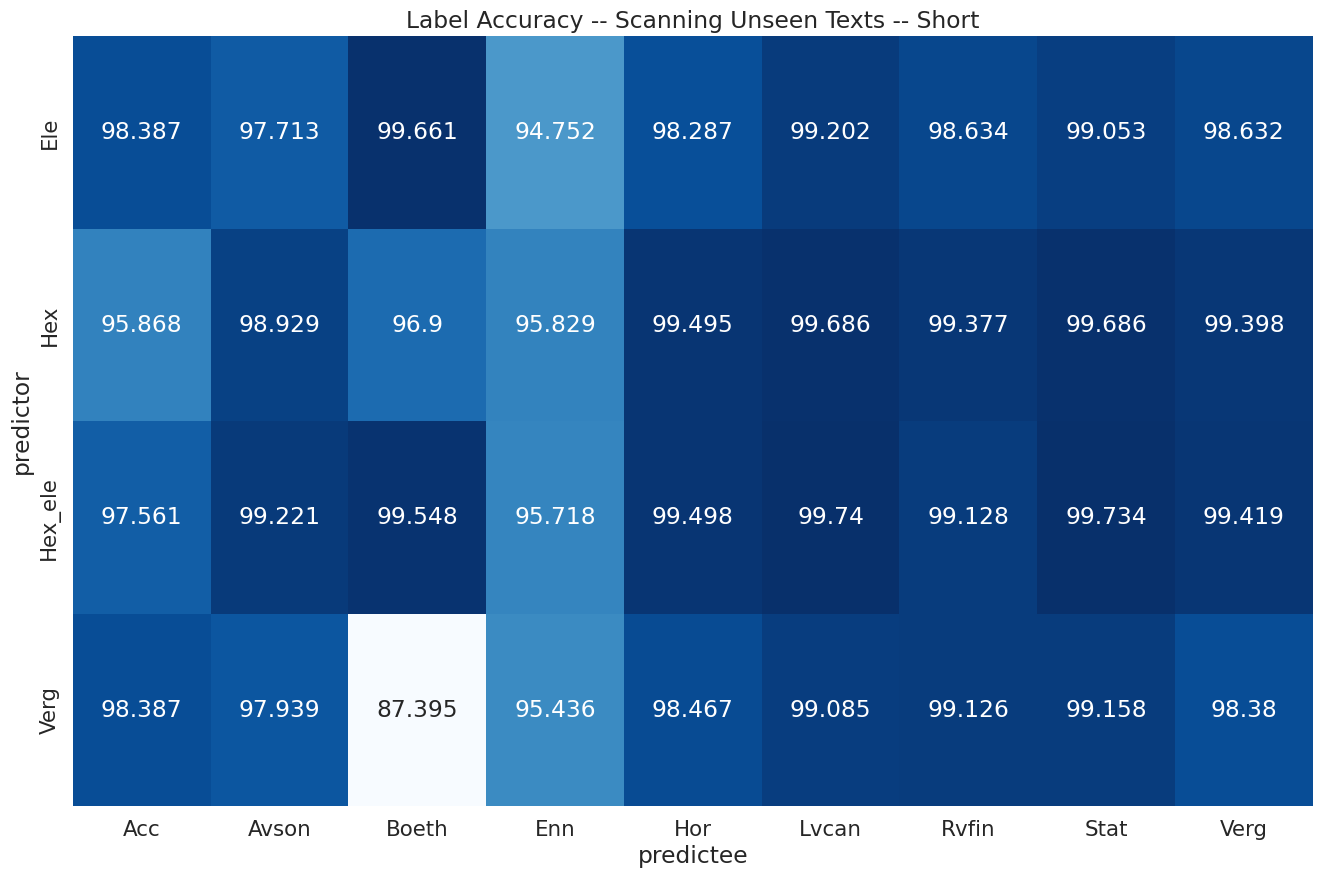
\includegraphics[width=0.48\textwidth]{img/lstm/lstm_unseen_texts-short.png}

    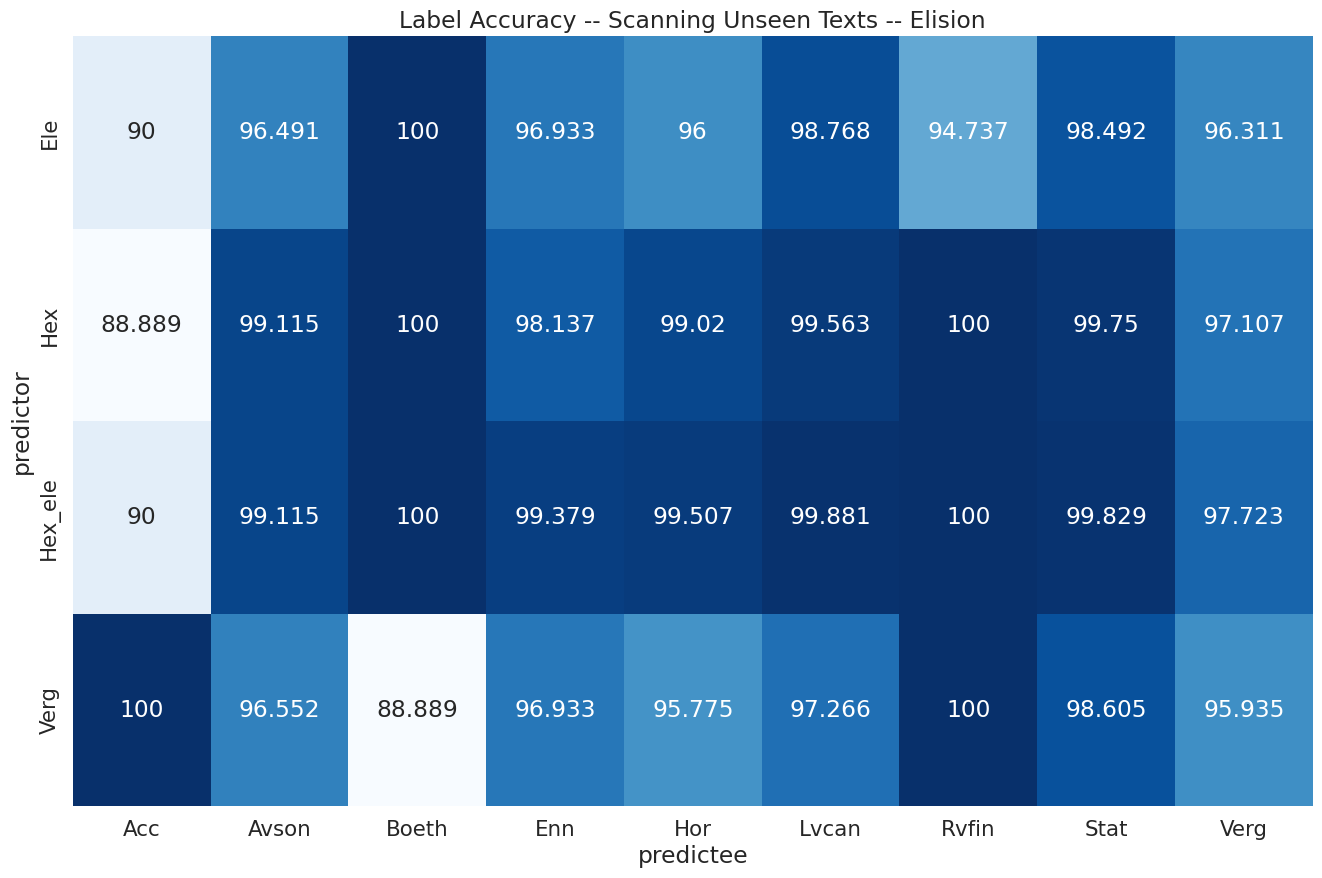
\includegraphics[width=0.48\textwidth]{img/lstm/lstm_unseen_texts-elision.png}
        % \quad
        % \includegraphics[width=0.48\textwidth]{img/task1_loss.png}

    % \captionsetup{justification=centering}
		\caption{LSTM label accuracy when combining hexameter and elegiac texts. Testing on unseen texts.}
    \label{fig:exp_architecture}
\end{figure}

\begin{table}[h]
\centering
    \begin{tabular}{||c c c c ||} 
     \hline
     Author & Text & Length & Verse \\ [0.5ex] 
     \hline\hline
        Catullus & Carmina &795 & H P\\
        Iuvenalis & Saturae & 833 & H\\
        Lucretius & De Rerum Natura & 7365 & H\\
        Ovidius & Metamorphoses & 11983 & H\\
        Persius & Saturae & 649 & H\\
        Vergilius & Aeneid & 9840 & H\\ %[1ex]
        \hline
        Propertius & Elegiae & 3998 & H P\\
        Tibullus & Elegiae & 1420 & H P\\
        Ovidius & (Elegiae) & 18832 & H P\\
        \hline
        Accius & Annalium fragmenta & 9 & H\\
        Ausonius & Ordo urbium nobilium & 168 & H\\
        Boethius & Consolatio Philosophiae & 76 & H P\\
        Ennius & Annalium fragmenta & 422 & H\\
        Horatius & Ars poetica & 476 & H\\
        Lucanus & Pharsalia & 8059 & H\\
        Rufinus & De numeris oratorum & 67 & H\\
        Statius & Thebais & 9739 & H\\
        Vergilius & Eclogae & 829 & H\\
     \hline

    \end{tabular}
    \caption{Table of texts and their lengths.}
    \label{table:1}
    % \label{fig:exp_architecture}
\end{table}

\begin{table}[h]
\centering
    \begin{tabular}{||c c c c ||} 
     \hline
      & LONG & SHORT & ELISION \\ [0.5ex] 
     \hline\hline
        ELE & 59.6 & 45.5 & 87.5\\
        HEX & 62.2 & 35.3 & 90.1\\
        HEX ELE & 62.6 & 39.5 & 90.1\\
        VERG & 58.1 & 28.5 & 88.4\\ [1ex]
     \hline

    \end{tabular}
    \caption{LSTM Accuracy on Seneca (Iambic Trimeter).}
    \label{table:2}
    % \label{fig:exp_architecture}
\end{table}

\begin{figure}[H]
    \centering
    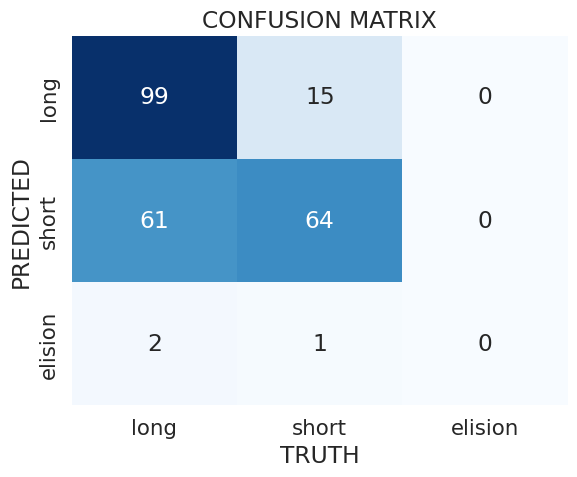
\includegraphics[width=0.6\textwidth]{img/lstm/lstm_confusion_matrix_trimeter_model.png}

    \caption{LSTM confusion matrix trained on iambic trimeter set (200 lines).}
    \label{fig:exp_architecture}
\end{figure}

\subsection{FLAIR}
